\chapter{Related Work}

Robotic manipulation and grasping is a field that has been extensively studied for decades via magnitude of different approaches. This chapter outlines some of the notable methods, while mainly focusing on contributions that employ model-free reinforcement learning due to their relevance for this project.


\section{Analytical Approaches}

% Analytical approaches in general
Analytical approaches determine grasps that satisfy target requirements through kinematic and dynamic formulations \cite{sahbani_overview_2012}. These methods typically analyze the geometry of target object and utilised gripper in order to generate a suitable grasp pose, which can then be reached by using a separate motion planner. The approach was introduced by \citet{nguyen_constructing_1987} through formulation of objectives for constructing stable force-closure grasps on polyhedral objects. By modelling objects as triangular mesh or 3D point cloud, force-closure grasps were later extended to remove model restrictions \cite{yun-hui_liu_complete_2004}. Several analytical metrics for estimating the quality of grasps were also introduced over the years to quantify good grasps \cite{roa_grasp_2015}, many of which have found their applicability beyond analytical approaches.

% Difficulties
Expert human knowledge of robot in a specific task is required to develop these algorithm, which allows them to achieve very efficient operation on a number of selected objects due to direct transfer of this knowledge. However, this also introduces a limitation because performance is restricted only to the predicted situations and scalable generalisation to novel objects is often unfeasible due to computation complexity that arises from the number of considered conditions \cite{sahbani_overview_2012}. Moreover, geometric models of objects might not be available before interaction is required, and partial occlusion of objects in setups with passive perception similarly limits the use of geometrical analysis.


\section{Supervised Learning}

% Empirical methods intro, reinforcement learning in general
Empirical methods were introduced to overcome shortcomings and difficulties of analytical approaches by combining sampling and training to achieve learning, which in turn reduces or removes the need to manually develop a model. A common approach is to use supervised learning to detect grasp poses by training on a dataset that is labelled with indication about what regions contain grasps \cite{saxena_robotic_2008, lenz_deep_2015}. Alternatively, a combination of analytical grasp quality metrics can be used to provide a more fine-tuned labelling of data \cite{mahler_dex-net_2017, mahler_dex-net_2018, mahler_learning_2019, lundell_robust_2019}. \citet{saxena_robotic_2008} applied supervised learning for detection of grasps on previously unseen objects by using handcrafted features from two or more RGB images of the scene in order to identify points in each image that correspond to grasp locations. They then determined the 3D position of detected grasps via triangulation and used custom heuristics to estimate orientation before planning a collision-free path.

% Intro to DL
Due to the significant advancements of deep learning (DL) in recent years, there has been a trend towards applying DL for robotic grasping. \citet{lenz_deep_2015} developed a framework that used DL to train two separate neural networks (NNs) on RGB-D data, where a small network was used to search for image patches with potential grasp candidates, and a larger network then ranked these candidates to select the most optimal grasp. With this work, \citeauthor{lenz_deep_2015} demonstrated the advantage of using DL instead of time-consuming design of hand-crafted features for robotic grasping. Popularity of convolution neural networks (CNNs) in computer vision applications also inspired their use for robotic grasping, which resulted in more accurate systems for predicting grasps in RGB-D images \cite{redmon_real-time_2015, kumra_robotic_2017}. The use of CNN also provides computationally efficiency, which allowed \citet{morrison_closing_2018} to synthesize grasps from depth images in real-time and perform closed-loop control.

% Supervised learning with 3D data representation
Besides 2D images, supervised DL methods have also been applied to 3D data representations. Approach by \citet{ten_pas_grasp_2017} randomly samples a large number of grasp candidates uniformly from the object surface using a point cloud, without a need to segment the individual objects first. They subsequently encode a region of interest around each grasp candidate as a stacked multi-channel projected image, which is then scored by the use of CNN classifier. By selecting the grasp candidate with the highest score, they were able to demonstrate a success rate of 93\% on novel objects in a dense clutter. \citet{lundell_robust_2019} used DL on voxel grid for shape completion of partially observed objects in order to obtain multiple predictions of the full object shape. These predictions were then used to jointly evaluate analytical grasp metrics for all grasp candidates, which they sampled from a mesh constructed as mean of all shape predictions. With this work, \citeauthor{lundell_robust_2019} demonstrated improved success rate over methods using only a partial view or a single shape estimate.

% Difficulties
Although supervised learning approaches can achieve high success rate, their main disadvantage is the large volume of labelled data required to effectively learn grasp generation. The process of labelling a dataset is generally automated because it is non-trivial to perform it manually due to the multitude of ways in which an object can be grasped, furthermore, human labelling introduces bias \cite{pinto_supersizing_2015}. However, the data collection itself is still very costly if performed on a physical setup. \citet{levine_learning_2016} used up to fourteen robots to collect 800,000 grasp attempts over the course of two months. To avoid this time-consuming process, majority of recent work relies on synthetically generated datasets. As an example, \citet{mahler_dex-net_2017} achieved 99\% precision by training on a dataset with 6.7 million point clouds of more than 10,000 unique 3D models, each containing grasps and corresponding analytical grasp metrics. Generalization to other gripper types is also limited and the entire dataset needs to be updated in order to support new types, which is why they created a new dataset of 2.8 million point clouds in \citeyear{mahler_dex-net_2018} for vacuum-based grippers. This issue was later addressed by creating a common dataset for both parallel-jaw and vacuum-based grippers by using a more complex and general analytical metric based on object's expected resistance to forces and torques \cite{mahler_learning_2019}.


\section{Imitation Learning}

% Imitation learning in general
Another empirical method is based on the process of learning tasks from demonstrations, called imitation learning. Demonstrations are normally represented as trajectories that contain states or state-action pairs, which can be obtained in several different ways such as teleoperation, kinesthetic teaching, or motion capture \cite{osa_algorithmic_2018}. In this way, imitation learning aims to provide robots with a desired behaviour by simply showing a sequence of actions instead of manually programming them.

% Behavioural cloning, short mention of LfO
Behavioural cloning is the simplest form of imitation learning, in which a policy that directly maps states to actions is learned through techniques such as non-linear regression or support vector machines \cite{osa_algorithmic_2018}. Recently, \citet{zhang_deep_2018} showed that DL allows behavioural cloning to be an effective way for robots to acquire complex skills. They used a virtual reality headset and hand-tracking controller to acquire teleoperated demonstrations in the form of RGB-D images, which were subsequently used to train a deep policy by the use of CNN. With this approach, \citeauthor{zhang_deep_2018} managed to train a simple grasping task with one object to 97\% success rate while using 180 distinct demonstrations. An emerging category termed learning from observation (LfO) aims to learn policy similarly from visual demonstrations that however do not have any labels associated with them and the state might not be fully known \cite{kroemer_review_2021}.

% Difficulties
Even though imitation learning provides a quick way of acquiring new policies, demonstrations usually do not contain all possible states that the robot might experience because collecting expert demonstrations for all scenarios can become too expensive and time-consuming \cite{osa_algorithmic_2018}. For this reason, the learned policy might struggle to generalize to novel objects and situations.


\section{Reinforcement Learning}

% RL in general, comparison with supervised and imitation learning, introduction to DRL
Reinforcement learning (RL) \cite{sutton_reinforcement_2018} aims to learn an optimal policy that maximises the total reward that is accumulated during sequential interaction with the environment. Unlike supervised and imitation learning, RL does not require any labelled datasets or demonstrations. Instead, RL agent collects information about the goal its trying to reach through direct interaction with the environment, all while improving its own policy. This process makes RL algorithms heavily dependent on reward signals, which is why it is important to design a reward function that induces learning towards reaching the desired goal. In addition to the popular benchmarks such as board- and video games that are commonly used to develop and test new algorithms, RL has been applied to several manipulation tasks over the years. Recently, the combination of DL and RL termed deep reinforcement learning (DRL) has become a popular choice for end-to-end control in robotics research, where sequential actions are learned directly from raw input observations.

% Model-based vs model-free
RL algorithms can be categorised depending on whether a model of the environment transition dynamics is used, i.e. model-based or model-free methods. Model-based RL algorithms have access to the model or learn it during the training, which allows the agent to predict state transitions and use such knowledge to directly learn the policy \cite{polydoros_survey_2017}. If the model is correct, model-based RL allows the learning process to be much more sample efficient than any model-free method, which gives model-based RL algorithms a great potential for applications within robotics. From this category, Probabilistic Inference for Learning Control (PILCO) \cite{deisenroth_pilco_2011} is model-based framework that has been applied also for manipulation tasks. With only 90 seconds of experience, \citet{durrant-whyte_learning_2012} applied PILCO to learn stacking task while incorporating collision avoidance into the planning. However, accurate models are rarely available and learning them can be very challenging in complex manipulation environments. Another difficulty emerges if an agent is trained and utilised in two different domains, which introduces bias to the model and ultimately leads to sub-optimal performance. For this reason, it might be significantly easier to learn a policy with model-free RL than to use model-based RL to learn transition dynamics, while achieving a similar level of performance \cite{kroemer_review_2021}. Therefore, the rest of this section will focus on contributions that use model-free methods to empirically learn a policy entirely from experience that is acquired via trial-and-error.

% RL in grasping, number of objects (generalisation)
The use of model-free DRL for robotic grasping has been explored by several works in last few years. Many of these contributions typically focus on the final performance using a single object \cite{popov_data-efficient_2017, haarnoja_composable_2018, zhan_framework_2020} or a limited number of objects with simple geometry such as boxes, cylinders or pyramids \cite{tobin_domain_2017, gualtieri_pick_2018, gualtieri_learning_2018, zeng_learning_2018, liu_active_2019, joshi_robotic_2020, daniel_deep_2020, iqbal_toward_2020}. More recent works strive to increase this variety by training on random objects with more complex geometry \cite{quillen_deep_2018, breyer_comparing_2019, wu_generative_2020, kim_acceleration_2020}, where the best diversity is achieved by training directly on real robots \cite{kalashnikov_qt-opt_2018}. Training on diverse objects allows DRL agent to learn a policy that provides the required generalisation, which is considered to be one of the most important challenges for learning-based robotic grasping \cite{quillen_deep_2018}.

% Action space
Contributions that apply DRL to robotic grasping also differ considerably in the utilised action space, where two main categories of approaches can be observed. The first category is based on pixel-wise action space \cite{zeng_learning_2018, gualtieri_learning_2018, liu_active_2019, daniel_deep_2020, wu_generative_2020}, in which the agent selects a pixel from the observed images in order to determine the position where an action primitive should be executed. The individual pixels are usually mapped to positions in Cartesian space and the action primitive is normally the entire grasp trajectory. Grasp orientation around vertical axis is commonly discretised by extending the action space to a set of images that are uniformly rotated copies of the original image \cite{zeng_learning_2018, daniel_deep_2020}. Orientation was extended to 3D by \citet{wu_generative_2020} via three image channels for continuous roll, pitch and yaw (RPY) angles. These action primitives can also be applied for other skills such as pushing, which \citet{zeng_learning_2018} used to allow agent to disturb objects before grasping them in order to clear space for fingers in scenes with densely packed objects. The second category of approaches in terms of action space are those that directly control robot motion \cite{quillen_deep_2018, kalashnikov_qt-opt_2018, breyer_comparing_2019, joshi_robotic_2020, zhan_framework_2020, kim_acceleration_2020, iqbal_toward_2020}, which is often expressed as Cartesian displacement of gripper pose in terms of relative translation $(d_x, d_y, d_z)$ and relative vertical rotation $d_\phi$. Control of the full 3D orientation in this way is uncommon, which is presumably due to the significantly increased complexity of such problem. However, there are works that directly control joints without the use of Inverse Kinematics (IK), e.g. \citet{popov_data-efficient_2017} uses continuous joint velocities. The gripper action also differs within this category, where some approaches automatically close the gripper after moving below certain height \cite{quillen_deep_2018} and others allow only closing of the gripper which subsequently terminates the episode \cite{kalashnikov_qt-opt_2018, joshi_robotic_2020}. A special formulation of action space was introduced by \citet{gualtieri_pick_2018}, where actions are grasp pose candidates sampled by the use their previous work \citet{ten_pas_grasp_2017}. Similar approach was adopted by \citet{osa_experiments_2017} for multi-finger grippers with a policy that also selected a grasp type in addition to grasp pose.

% Observation space
Although the observation space is for some manipulation tasks defined in form of states extracted from the simulation, e.g. gripper and object position \cite{popov_data-efficient_2017, haarnoja_composable_2018}, the vast majority of RL grasping research relies on visual image observations that are combined with CNNs. Among these are RGB image \cite{tobin_domain_2017, kalashnikov_qt-opt_2018, quillen_deep_2018, kim_acceleration_2020, iqbal_toward_2020}, depth map \cite{gualtieri_learning_2018, breyer_comparing_2019, wu_generative_2020} or RGB-D \cite{zeng_learning_2018, liu_active_2019, daniel_deep_2020}. A single camera is commonly mounted statically in the environment and the preprocessing of images is usually very minimal. \citet{zhan_framework_2020, joshi_robotic_2020} utilised two cameras simultaneously, where the first is mounted statically in the environment and the second is attached to the gripper. Despite the dominant use of 2D visual observations, the use of 3D data representation for RL grasping is currently very limited. Even though some works use point clouds as an intermediate representation \cite{zeng_learning_2018, gualtieri_learning_2018}, these are subsequently projected into one or more 2D image views that are then individually processed by a CNN. \citet{osa_experiments_2017, gualtieri_pick_2018} also utilise point clouds but only to sample grasp candidates with non-RL methods, where RL policy is then used to select one of them. Based on this investigation, there is a general lack of methods for robotic grasping that utilise RL for end-to-end control with visual observations that are represented in 3D. The primary reason for this is presumably the popularity of existing deep learning frameworks that allow efficient use of CNN to extract features from 2D images for DRL. However, it can be argued that convolutional layers do not provide the desired level of generalisation over depth information and spatial orientation compared to their well-established generalisation for horizontal and vertical position in the image \cite{gualtieri_pick_2018}, even if applied to 2.5D data representation in form of depth map or aligned RGB-D images. Therefore, this work studies the importance of such generalisation over the full 6 DOF workspace in which robots grasp objects.

% Difficulties
Application of RL to real world robotics problems is still limited due to several difficulties. Sample inefficiency is especially problematic in robotics because it can take few minutes to collect a single training sample of grasping on a real robot. One way to collect more data is by using multiple robots simultaneously. For example, \citet{kalashnikov_qt-opt_2018} used seven robots to collect 580,000 grasps over the course of several weeks, which can become very costly and unpractical. Moreover, the exploratory nature of RL is unsafe and induces jerky motion patterns, which leads to mechanical wear and potential damage of the actuators \cite{kroemer_review_2021}. Therefore, use of synthetic data in form of robotics simulators is common among RL research because it greatly improves the availability of training data. Similar to real robots, running multiple simulation workers in parallel can also accelerate the rate at which data is collected, e.g. \citet{popov_data-efficient_2017} used 16 such virtual workers. However, there is a reality gap between simulation and real robot data which must be addressed. Some of the most common Sim2Real approaches to achieve this transition will be described in \autoref{subsec:sim2real}. Reproducibility of state-of-the-art RL methods is also not very straightforward, as robotics environments are rarely deterministic and performance of RL methods can be highly influenced by many factors such as selection of hyperparameters and scaling of the reward \cite{henderson_deep_2018}. Random seed that is used to initialise pseudorandom generator during training can also have a significant influence on the learning curve and final performance as visualised in \autoref{fig:reproducibility_random_seed}. These issues are further magnified by robot and hardware requirements in addition to any use of proprietary software or framework, hence simulated setup with open-source software is highly preferred for RL research.

\begin{figure}[ht]
    \centering
    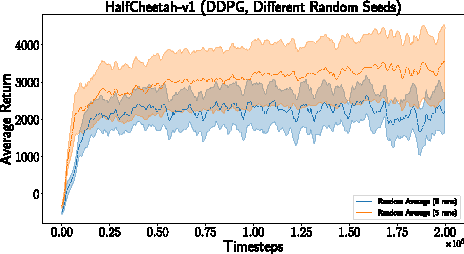
\includegraphics[width=0.667\textwidth]{related_work/reproducibility_random_seed.pdf}
    \caption{Learning curve of DDPG on a locomotion environment for two sets of five different random seeds. All runs use the same hyperparameter configuration. \cite{henderson_deep_2018}}
    \label{fig:reproducibility_random_seed}
\end{figure}


\subsection{Sim2Real}\label{subsec:sim2real}

Due to the popularity of training DRL agents inside simulations, there are several approaches that have been applied to bridge the reality gap and achieve Sim2Real transfer without any retraining. The most straightforward approach is to reduce or completely eliminate such gap by utilising a realistic simulation software that can correctly simulate the required physical interactions and provide visualisation based on principles of physically based rendering (PBR). For example, \citet{iqbal_toward_2020} developed a robotics simulator with a physics solver on top of game engine that provides photorealistic rendering. However, there is a computational cost connected with such realism and compromises must be made in order to achieve a desired rate at which training data can be effectively produced. Consequently, other methods that increase the variety in the data have been utilised over the years, with aim to provide a better generalisation that would make the learned policy applicable to real world. Some of these methods are useful even for realistic virtual environments as a mean to increase diversity due to their low computational cost.

\paragraph{Data Augmentation} The amount of available data can be increased by synthetically creating modified copies of the existing data. This approach is not only popular in supervised learning as a mean to enlarge dataset, but it has also been applied in RL \cite{zhang_towards_2015, laskin_reinforcement_2020, zhan_framework_2020}. In this context, data augmentation is commonly applied to the visual observations in form of 2D images with operations such as cropping, rotation, cut-out and adding jitter to the colour channels.

\paragraph{Domain Adaptation} Instead of reducing the reality gap at simulation level, domain adaptation modifies observations from source domain to provide a better resemblance in the target domain. \citet{zhang_towards_2015} applied this technique to generate synthetic images of robot arm that were similar to the training data based on real-time readings of robot's joint angle positions. In the opposite direction, \citet{bousmalis_using_2018} employed generative adversarial network (GAN) during training in order to adapt the synthetic images from simulation and make them closely resemble visuals of real-world domain, as illustrated in \autoref{fig:sim2real_domain_adaptation}.

\begin{figure}[ht]
    \centering
    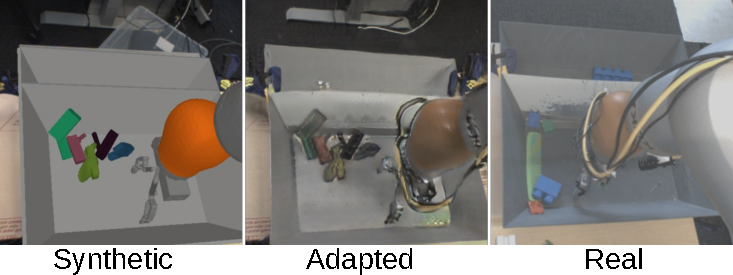
\includegraphics[width=0.75\textwidth]{related_work/sim2real_domain_adaptation.pdf}
    \caption{Example of domain adaptation applied to robotic grasping. \cite{bousmalis_using_2018}}
    \label{fig:sim2real_domain_adaptation}
\end{figure}

\paragraph{Domain Randomization} Another way to easily expand the variety in data is by randomly changing the simulated environment. \citet{tobin_domain_2017} applied this method in order to randomize visual attributes shown in \autoref{fig:sim2real_domain_randomization}, such as object colours, table texture, camera pose and characteristics of the illumination. Furthermore, domain randomization can be extended also to other non-visual simulation attributes such as inertial properties of robot links and hyperparameters of the utilised physics solver.

\begin{figure}[ht]
    \centering
    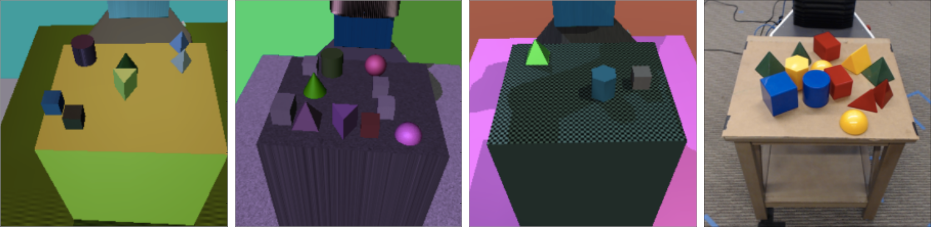
\includegraphics[width=1.0\textwidth]{related_work/sim2real_domain_randomization.png}
    \caption{Example of domain randomization for visual attributes. Corresponding image of real-world domain is shown on the right. \cite{tobin_domain_2017}}
    \label{fig:sim2real_domain_randomization}
\end{figure}

